\chapter{Peruskäsitteitä}
\section{Tyyppijärjestelmät}
Tyyppijärjestelmät, tai \textit{tyyppiteoria}, on tutkimusalue matematiikan
ja filosofian alalla \cite{TypesAndProgrammingLanguages}. Tarkka
\dblquoted{tyyppijärjestelmän} määritelmä riippuu siitä minkä
tieteenalan ja -haaran näkökulmasta sitä käsitellään. Tässä tutkielmassa
tyyppijärjestelmiä tarkastellaan käytännönläheisesti
ohjelmointikielten näkökulmasta metodina, jolla voidaan osoittaa
virheellisissä ohjelmissa olevia puutteita luokittelemalla
ohjelman rakenteita tyypeiksi ja vertaamalla niitä ohjelmointikielen
tyyppisääntöjä vasten. 

\section{Luokittelu}
Ohjelmointikielten tyyppijärjestelmien jakaminen staattisesti ja dynaamisesti
tyyppitarkastettuihin (puhekielessä usein: staattisesti ja dynaamisesti
\dblquoted{tyypitettyihin}) perustuu ohjelman kehitysvaiheeseen, jossa tarkastaminen
tapahtuu. Staattisella tyyppitarkastamisella viitataan ohjelman tyyppien
analyysiin ennen ohjelman suorittamista, esimerkiksi käännösaikana, kun taas
dynaaminen tyyppitarkastus varmistaa arvojen tyyppien oikeellisuuden ohjelmaa
suoritettaessa.

\begin{figure}
\centering
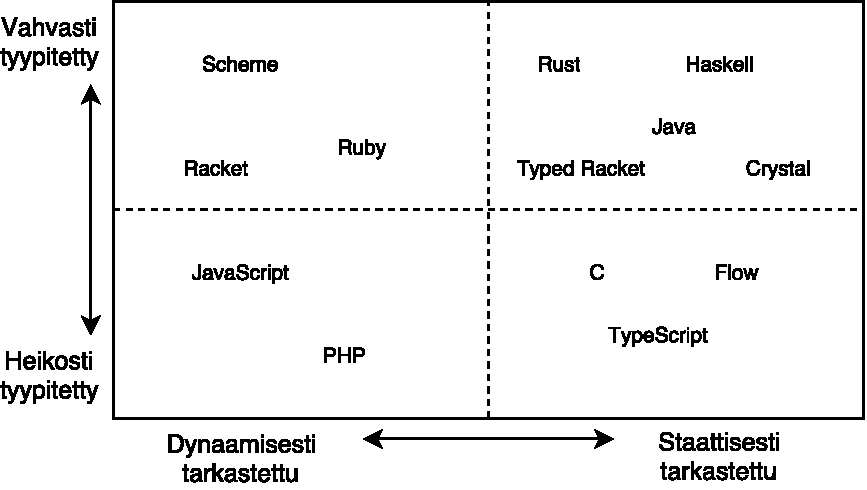
\includegraphics{images/type-systems.pdf}
\caption{Tyyppijärjestelmät eri ohjelmointikielissä}
\end{figure}

Esimerkiksi ohjelma \inlinecode{\dblquoted{teksti}.potenssiin(3)} antaa
staattisesti tyyppitarkastetussa kielessä virheen jo käännösaikana, mikäli
metodia \inlinecode{potenssiin} ei ole tekstityyppisille arvoille määritetty.
Staattisesti tyyppitarkastetussa kielessä muuttujien
mahdolliset tyypit analysoidaan käännösaikana, ennen ohjelman suorittamista.
Kääntäjä näkee, että lausekkeen vasen puoli, \inlinecode{\dblquoted{teksti}},
on tyypiltään teksti ja oikea puoli on metodin \inlinecode{potenssiin} kutsu.
Kääntäjä voi todeta kielen tyyppisääntöjen perusteella, ettei
tekstimuotoisessa arvossa ole metodia \dblquoted{potenssiin} ja
pysäyttää virheellisen ohjelman käsittelyn.

Tyyppijärjestelmät voidaan jaotella myös muiden
ominaisuuksien perusteella esimerkiksi vahvoihin ja heikkoihin
tyyppijärjestelmiin. Näiden termien merkitys ei ole tarkasti määritelty,
mutta yleisesti niillä viitataan tapaan, jolla kieli käsittelee tarkoitetusta
poikkeavat, virheelliset tyypit \cite{CornellTransitionToOO}. Vahvasti
tyypitetyssä kielessä tietyntyyppisen muuttujan vääränlainen käsittely
aiheuttaisi käännös- tai ajonaikaisen virheen, kun taas heikosti tyypitetyssä
kielessä arvolle voitaisiin tehdä implisiittisiä tyyppimuunnoksia niiden
yhteensopivuuden saavuttamiseksi.

JavaScript on dynaamisesti tarkastettu, heikosti tyypitetty kieli.
JavaScriptiä suorittava ympäristö hyväksyisi ohjelman ja sallisi
sen suorittamisen. Virhe olemattoman metodin kutsumisesta
ilmenisi vasta jos ohjelmaa testataan käytännössä ja
kyseinen virheen sisältävä osa koodia suoritetaan.
Lisäksi esimerkiksi lausekkeen \inlinecode{\dblquoted{teksti} + 2}
laskeminen ei aiheuttaisi virhettä edes suoritusaikana, sillä heikoille
tyyppijärjestelmille ominaisesti JavaScript muuttaisi numeron 2 tekstimuotoon
ennen summausoperaation arviointia ja antaisi tulokseksi
\inlinecode{\dblquoted{teksti2}}, mikä ei välttämättä ollut koodin
alkuperäinen tarkoitus. Tässä tutkielmassa keskitytään lähinnä
JavaScriptin tyyppien staattiseen ja dynaamiseen, eli käytännössä
käännös- ja ajonaikaiseen tarkastamiseen. Eräät
esitellyistä työkaluista myös\newline
tiukentavat kielen sallimia operaatioita siten,
että esimerkiksi yllä esitettyä\newline
\inlinecode{\dblquoted{teksti} + 2} lauseketta
ei enää sallittaisi.

\section{EcmaScript ja JavaScript}
\textit{EcmaScript} on ECMA-262 standardin määrittelemä ohjelmointikieli
\cite{JavaScriptLanguageResources, Ecma262}, jonka kehityksestä vastaa
organisaatio Ecma International. \textit{JavaScript} puolestaan on Oraclen omistama
tavaramerkki jolla viitataan EcmaScript-kielen osittaisiin tai täydellisiin
toteutuksiin \cite{JavaScriptLanguageResources}. Historiallisista syistä termejä
``JavaScript'' ja ``EcmaScript'' käytetään usein keskenään vaihtokelpoisesti.
Tässä tutkielmassa termillä ``JavaScript'' viitataan ECMA-262-spesifikaation kahdeksannen
version mukaiseen EcmaScriptiin, jota kutsutaan myös nimellä EcmaScript 2017.

\section{TypeScript}
TypeScript on Microsoftin luoma ohjelmointikieli, jonka tarkoitus on
auttaa JavaScript-ohjelmien kehitystä staattisen tyyppijärjestelmän avulla.
Se on EcmaScriptin ylijoukko (engl. superset) \cite{TypeScriptSpec} ja jatkaa
JavaScriptin syntaksia tyyppimäärittelyihin käytettävällä
annotaatiosyntaksilla. Jokainen validi JavaScript-ohjelma on syntaksiltaan ja
ajonaikaiselta käyttäytymiseltään validi TypeScript-ohjelma. TypeScript
kuitenkin lisää kehitykseen käännösvaiheen, jossa ohjelman tyyppien
oikeellisuus tarkastetaan staattisesti. TypeScript-koodi käännetään
JavaScriptiksi, joka puolestaan voidaan suorittaa selaimissa tai muissa
JavaScriptin suoritusympäristöissä. TypeScript-kääntäjän voi myös määrittää
muokkaamaan tulostettava koodi yhteensopivaksi vanhojen
EcmaScript-standardien kanssa, mikä on hyödyllistä, jos ohjelman on tarkoitus
tukea sellaisia suoritusympäristöjä, jotka eivät tue uusinta EcmaScriptin
versiota.

\section{Flow}
Flow on Facebookin kehittämä työkalu, joka TypeScriptin tavoin jatkaa
JavaScriptin syntaksia staattisesti tarkastettavilla tyyppimäärittelyillä.
Flow itsessään ei sisällä kääntäjää, vaan keskittyy yksinomaan ohjelman
tyyppiturvallisuuden tarkastamiseen. Koodiin lisätyt tyyppimääritykset on
kuitenkin poistettava ennen kuin JavaScript-ohjelma voidaan suorittaa. Tähän
tarkoitukseen voidaan käyttää esimerkiksi Babel-kääntäjää, joka poistaa
Flow-tyyppimäärittelyt ja muokkaa JavaScript-koodin yhteensopivaksi toivotun
EcmaScript-version kanssa \cite{FlowInstallation}.

\section{Closure}
Googlen Closure-kääntäjä on käännöstyökalu, jonka pääasiallinen tarkoitus
on minimoida ja optimoida JavaScript-koodia käännösvaiheessa ennen tuotantoon
siirtämistä. Closure sisältää kuitenkin myös tuen tyyppivirheiden
tarkastamiselle käännösvaiheessa \cite{ClosureCompiler}. Tyypit annotoidaan
erityisellä JSDoc-pohjaisilla dokumentaatiokommenteilla. Koska annotaatiot
ovat kommenteissa eivätkä erityisenä syntaksina muun suoritettavan koodin
joukossa, Closure-annotoitua JavaScriptiä ei tarvitse kääntää ennen sen
suorittamista \cite{annotatingJSforClosure}. Kehittäjä voi suorittaa koodin
sellaisenaan ilman aikaavievää käännösprosessia. Kun ohjelma on valmis,
se voidaan haluttaessa ajaa Closure-kääntäjän läpi tiedostokoon
ja suoritusnopeuden optimoinniksi.
